\begin{figure}[htbp]
\centering
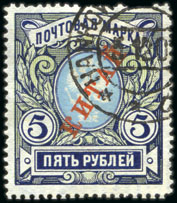
\includegraphics[width=.30\textwidth]{../russian-post-offices-in-china/10114.jpg}
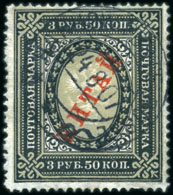
\includegraphics[width=.30\textwidth]{../russian-post-offices-in-china/10114-1.jpg}
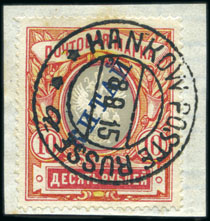
\includegraphics[width=.30\textwidth]{../russian-post-offices-in-china/10114-2.jpg}
\caption{ 
10114 HANKOW: Small selection of stamps incl. T\&S type 2A on \$1 on 
1R (minor faults), type 3A on "KITAI" 1k block of four and on 10R, and type 3B 
on "KITAI" 3R50 and 5R, fine group

(Image 1) (Image 2) (Image 3)	
\euro100.00 
} 
\end{figure} 

\begin{figure}[htbp]
\centering
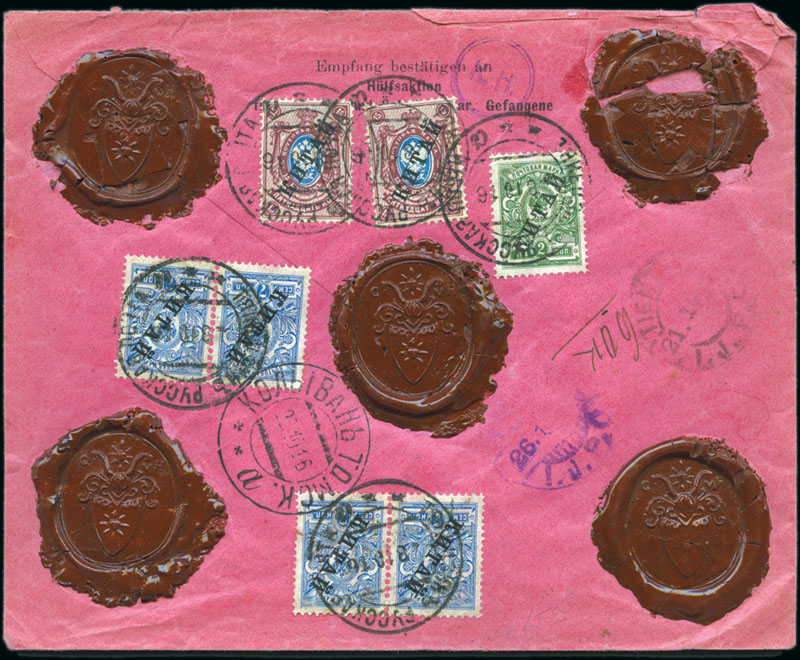
\includegraphics[width=.95\textwidth]{../russian-post-offices-in-china/10015.jpg}
\caption{ 
10115	HANKOW: 1908 Cover sent registered to Krakow (Austria, now in Poland), 
with "KITAI" 3k (2) and 20k tied by Hankow 15.6.08 cds (T\&S type 3A), with 
rare registered label in English adjacent, slight soiling and missing backflap.
\euro 400.00 
} 
\end{figure} 

\begin{figure}[htbp]
\centering
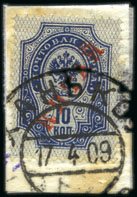
\includegraphics[width=.35\textwidth]{../russian-post-offices-in-china/10116.jpg}
\caption{ 
10116 HANKOW: "KITAI" 10k on VERTICALLY LAID PAPER, tied on piece by Hankow
17.4.09 cds (T\&S type 2), very rare as only a few sheets of the 10k on 
vertically laid paper were accidentally overprinted "KITAI".
\euro 800.00 
} 
\end{figure}   
  
\begin{figure}[htbp]
\centering
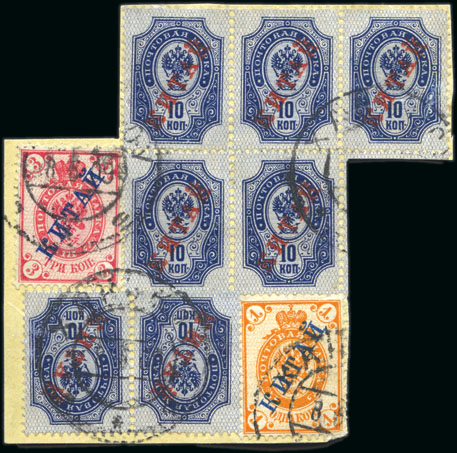
\includegraphics[width=.95\textwidth]{../russian-post-offices-in-china/10117.jpg}
\caption{ 
10117 HANKOW: Piece with seven "KITAI" 10k on VERTICALLY LAID PAPER 
(in block of five and pair) plus 1k and 3k, tied by Hankow 8.5.09 cds 
(T\&S type 2), a rarity and a magnificent multiple, as only a few sheets 
of the 10k on vertically laid paper were accidentally overprinted "KITAI", 
signed Holcombe and Calves

Provenance: Ex Lipschutz and Mizuhara
\euro 8,000.00
} 
\end{figure}   
  
  
\begin{figure}[htbp]
\centering
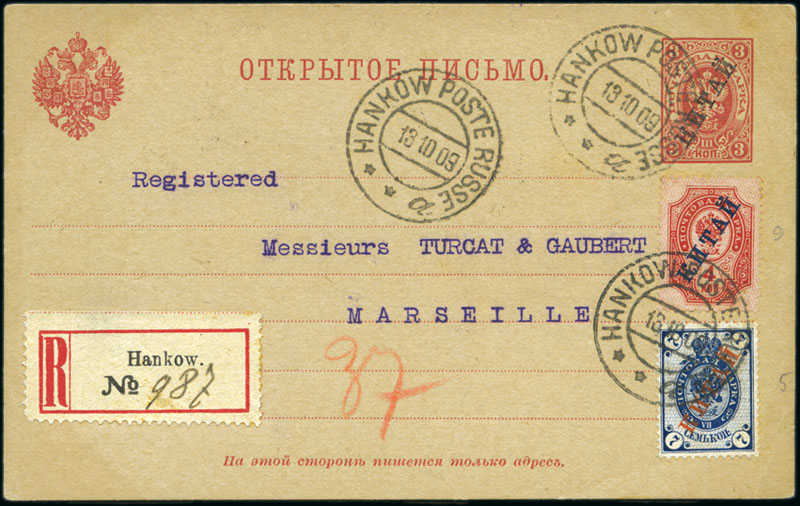
\includegraphics[width=.95\textwidth]{../russian-post-offices-in-china/10118.jpg}
\caption{ 
10118 HANKOW: 1909 "KITAI" 3k postcard to France, uprated with "KITAI" 4k and 7k, 
all cancelled by Hankow 13.10.09 cds (T\&S type 3A), reg'd label in 
English adjacent, Marseille bs, very fine and neat.
\euro 400.00
} 
\end{figure}   
  
  
\begin{figure}[htbp]
\centering
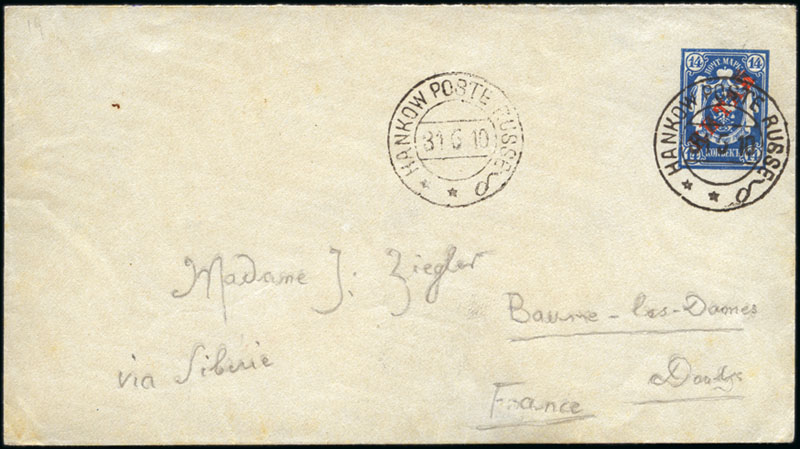
\includegraphics[width=.95\textwidth]{../russian-post-offices-in-china/10119.jpg}
\caption{ 
10119 HANKOW: 1910 "KITAI" 14k postal stationery envelope sent to France, 
cancelled by Hankow 31.5.10 cds (Tchilinghirian type 3B), Baume-Les-Dames bs, 
probably a philatelic usage as it is overpaying the 10k foreign letter 
rate, still a scarce usage of this stationery.
\euro 100.00
} 
\end{figure}   
  
\begin{figure}[htbp]
\centering
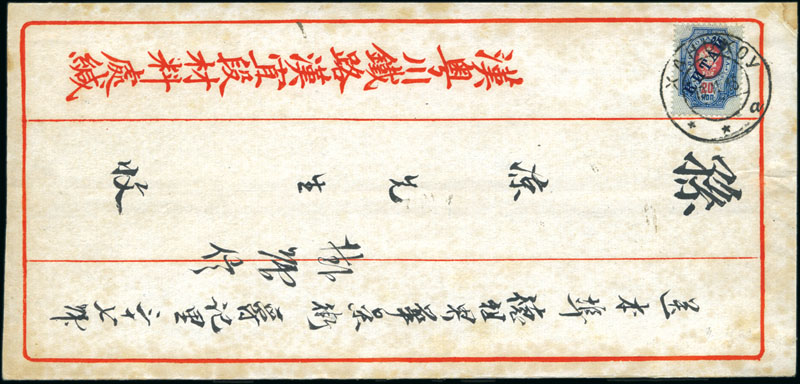
\includegraphics[width=.95\textwidth]{../russian-post-offices-in-china/10120.jpg}
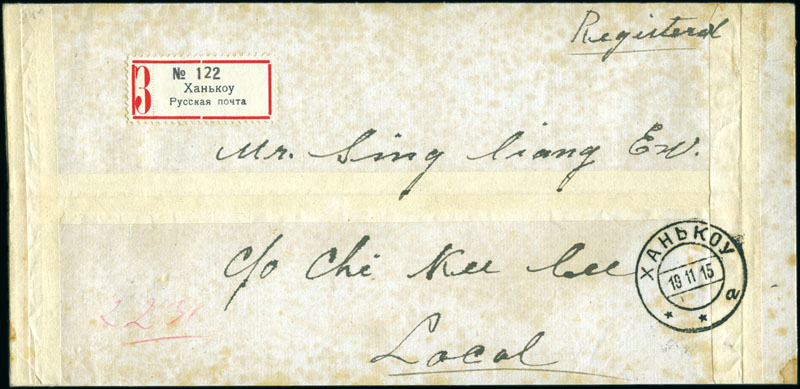
\includegraphics[width=.95\textwidth]{../russian-post-offices-in-china/10120-1.jpg}
\caption{ 
10120 HANKOW: 1915 Native cover registered locally in Hankow with "KITAI" 20k 
tied by Hankow 19.11.15 cds (T\&S type 2a), reg'd label in Cyrillic on reverse,
opened for display and some foxing, still an unusual use of the Russian P.O.
for local delivery
\euro 400.00 
} 
\end{figure}   
  
\begin{figure}[htbp]
\centering
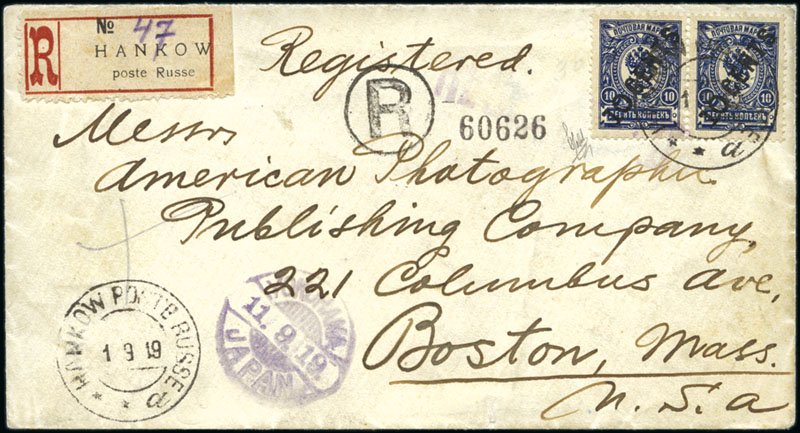
\includegraphics[width=.95\textwidth]{../russian-post-offices-in-china/10121.jpg}
\caption{ 
10121 HANKOW: 1919 Cover registered to the USA with Russia Chinese surcharged 10c
on 10k pair tied by Hankow 1.9.19 cds (T\&S type 3A), with reg'd label in French 
and encircled "R" hs adjacent, Yokohama transit and Boston bs, a very fine 
and late use from the Hankow office with a franking seldom seen from there,
signed Holcombe.

Note: The Russian P.O. at Hankow was closed November 1920
\euro 400.00
} 
\end{figure}    

\begin{figure}[htbp]
\centering
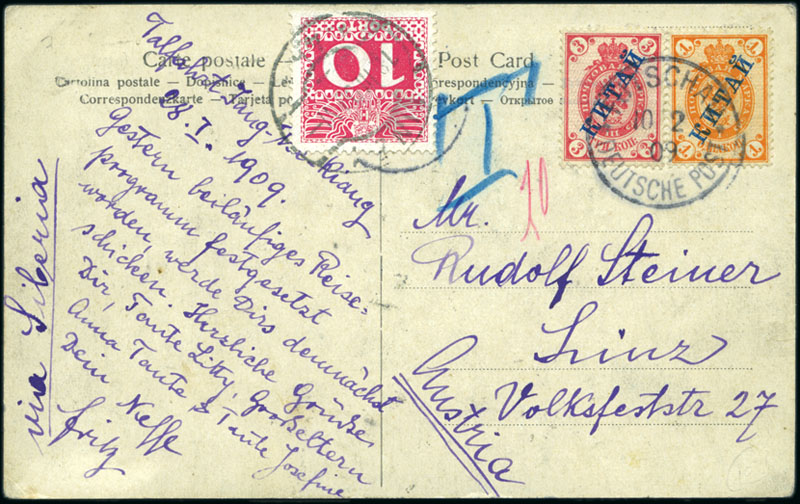
\includegraphics[width=.95\textwidth]{../russian-post-offices-in-china/10122.jpg}
\caption{ 
10122 GERMAN POST IN FOOCHOW: 1909 Picture postcard of Nanking to Austria with 
"KITAI" 1k and 3k tied by German P.O. "FUTSCHAU" 10.2.09 cds, however since 
Russian stamps were invalid at this Office the card was marked with "T" and "10" 
and had a 10h postage due added on arrival in Linz, very unusual
\euro 400.00 
} 
\end{figure}  




  
  
                                  